% This is samplepaper.tex, a sample chapter demonstrating the
% LLNCS macro package for Springer Computer Science proceedings;
% Version 2.21 of 2022/01/12
%
\documentclass[runningheads]{llncs}
%
\usepackage[T1]{fontenc}
% T1 fonts will be used to generate the final print and online PDFs,
% so please use T1 fonts in your manuscript whenever possible.
% Other font encondings may result in incorrect characters.
%
\usepackage{graphicx}
% Used for displaying a sample figure. If possible, figure files should
% be included in EPS format.
%
% If you use the hyperref package, please uncomment the following two lines
% to display URLs in blue roman font according to Springer's eBook style:
%\usepackage{color}
%\renewcommand\UrlFont{\color{blue}\rmfamily}
%\urlstyle{rm}
%
\usepackage{lipsum}
\usepackage{amsmath}
\usepackage{amssymb}
\DeclareMathOperator*{\argmin}{arg\,min}
\usepackage{booktabs}
\usepackage{xcolor}
\usepackage{graphicx}
\usepackage{pgfplots}
\pgfplotsset{compat=1.18}

% ---------------------------------------------------------------
% Drafting helpers -- REMOVE BEFORE SUBMISSION
% ---------------------------------------------------------------
% Placeholder box standing in for a figure that does not exist yet.
% Usage: \figplaceholder{0.28}{what the figure will show}
\newcommand{\figplaceholder}[2]{%
  \fbox{\begin{minipage}[c][#1\textheight][c]{0.97\linewidth}%
    \centering\itshape\small #2%
  \end{minipage}}%
}
% Inline TODO marker.
\newcommand{\todo}[1]{\textcolor{red}{[TODO: #1]}}
% Journal-extension markup: switch to \journalbluefalse for black text.
\newif\ifjournalblue
\journalbluetrue
\newcommand{\journalcolor}{\ifjournalblue\color{blue}\fi}
\newcommand{\journal}[1]{{\journalcolor #1}}
\newenvironment{journaladdition}{\begingroup\journalcolor}{\endgroup}
% TODOs stay red; blue prose/bullets describe the planned journal study.

\begin{document}
%
\title{PET Quantification-Preserving Registration for Longitudinal Whole-Body PSMA PET/CT}
%
\titlerunning{Quantification-Preserving PSMA PET/CT Registration}
% If the paper title is too long for the running head, you can set
% an abbreviated paper title here
%
%\author{Fryderyk K{\"o}gl\inst{1}\orcidID{0000-0000-0000-0000} \and
%Anna Reithmeir\inst{2,3}\orcidID{1111-1111-1111-1111} \and
%Daniel M. Lang\inst{2,3}\orcidID{1111-1111-1111-1111} \and
%Emily Chan\inst{2,3}\orcidID{1111-1111-1111-1111} \and
%Rickmer Braren\inst{2,3}\orcidID{1111-2222-3333-4444} \and
%Julia A. Schnabel\inst{3}\orcidID{2222--3333-4444-5555}}
%%
%\authorrunning{F. K{\"o}gl et al.}
%% First names are abbreviated in the running head.
%% If there are more than two authors, 'et al.' is used.
%%
%\institute{Princeton University, Princeton NJ 08544, USA \and
%Springer Heidelberg, Tiergartenstr. 17, 69121 Heidelberg, Germany
%\email{lncs@springer.com}\\
%\url{http://www.springer.com/gp/computer-science/lncs} \and
%ABC Institute, Rupert-Karls-University Heidelberg, Heidelberg, Germany\\
%\email{\{abc,lncs\}@uni-heidelberg.de}}
\author{Anonymous Author(s)}
\authorrunning{Anonymous et al.}
\institute{Anonymous Institution(s)}
%
\maketitle              % typeset the header of the contribution
%
\begin{abstract}

\begin{journaladdition}
We investigate how PET biomarker preservation and bone rigidity affect longitudinal whole-body PSMA PET/CT registration.
The study uses a LapIRN pipeline with an affine stage and test-time instance optimization.
The planned evaluation separates the contributions of PET preservation and rigidity, compares existing rigidity penalties, and characterizes the trade-off between anatomical alignment and lesion-level quantification preservation.
\todo{Replace this prospective abstract after the independent evaluation: add patient counts, principal paired effects with uncertainty, and a conclusion supported by the results.}
\end{journaladdition}

\keywords{Deformable image registration \and PSMA PET/CT \and Longitudinal
imaging \and Biomarker preservation.}
\end{abstract}
%
%
%
\section{Introduction}

Prostate-specific membrane antigen (PSMA) PET/CT has become a central imaging modality for staging, treatment planning, radiopharmaceutical therapy, and post-therapy response assessment in prostate cancer~\cite{ref_psma_clinical}.
In these settings, patients often undergo multiple scans over time, comprising a baseline scan before therapy and one or more follow-up scans.
Accurate baseline-to-follow-up registration can support the comparison of disease burden, the localization of uptake changes, the assessment of lesion progression or response, dose accumulation, and quantitative longitudinal analysis~\cite{ref_psmareg_challenge}.
For such analyses, the deformation should align anatomy without introducing artificial changes in PET-derived tumor burden measures.
The Learn2Reg~2026 PSMAReg challenge~\cite{ref_learn2reg_alessa,ref_learn2reg_hansen,ref_psmaregdata} formalizes this problem as the estimation of a dense displacement field that warps each follow-up (moving) scan to its baseline (fixed) scan.
The challenge evaluates registration accuracy using organ overlap and boundary distance, deformation regularity, and preservation of two PET-derived biomarkers: metabolic tumor volume (MTV) and total lesion glycolysis (TLG).

Deformable registration can be formulated as iterative optimization of a regularized objective functional~\cite{ref_demons,ref_syn,bspline}, which can achieve high accuracy but is computationally demanding for whole-body images.
Learning-based methods instead amortize this optimization into network weights and replace per-pair iteration with a single forward pass at inference~\cite{ref_voxelmorph_cvpr,ref_svf_voxelmorph,ref_transmorph}.
We therefore build on LapIRN~\cite{ref_lapirn}, whose coarse-to-fine Laplacian pyramid is well suited to recovering the large deformations expected between longitudinal whole-body scans while maintaining smooth and invertible transformations.





\begin{journaladdition}
This journal study builds on our earlier registration pipeline and asks how PET preservation and bone rigidity affect alignment, lesion quantification, and deformation quality.
Preservation refers to changes introduced by warping the same scan; it does not require uptake or tumor burden to remain equal between longitudinal examinations.
\todo{Add the citation to the earlier paper and a concise statement of the journal extension.}
The study is organized around three questions:
\begin{itemize}
  \item What are the separate and combined effects of PET preservation and bone rigidity, and what does each PET loss term contribute?
  \item How do existing rigidity penalties compare in low-resolution whole-body CT, including their effects on bone shape and surrounding tissue?
  \item How does the strength of PET preservation change the balance between anatomical alignment, lesion preservation, and deformation quality?
\end{itemize}
The rigidity study evaluates existing approaches in this setting rather than introducing a new rigidity method.
\end{journaladdition}



\begin{figure}[t]
\centering
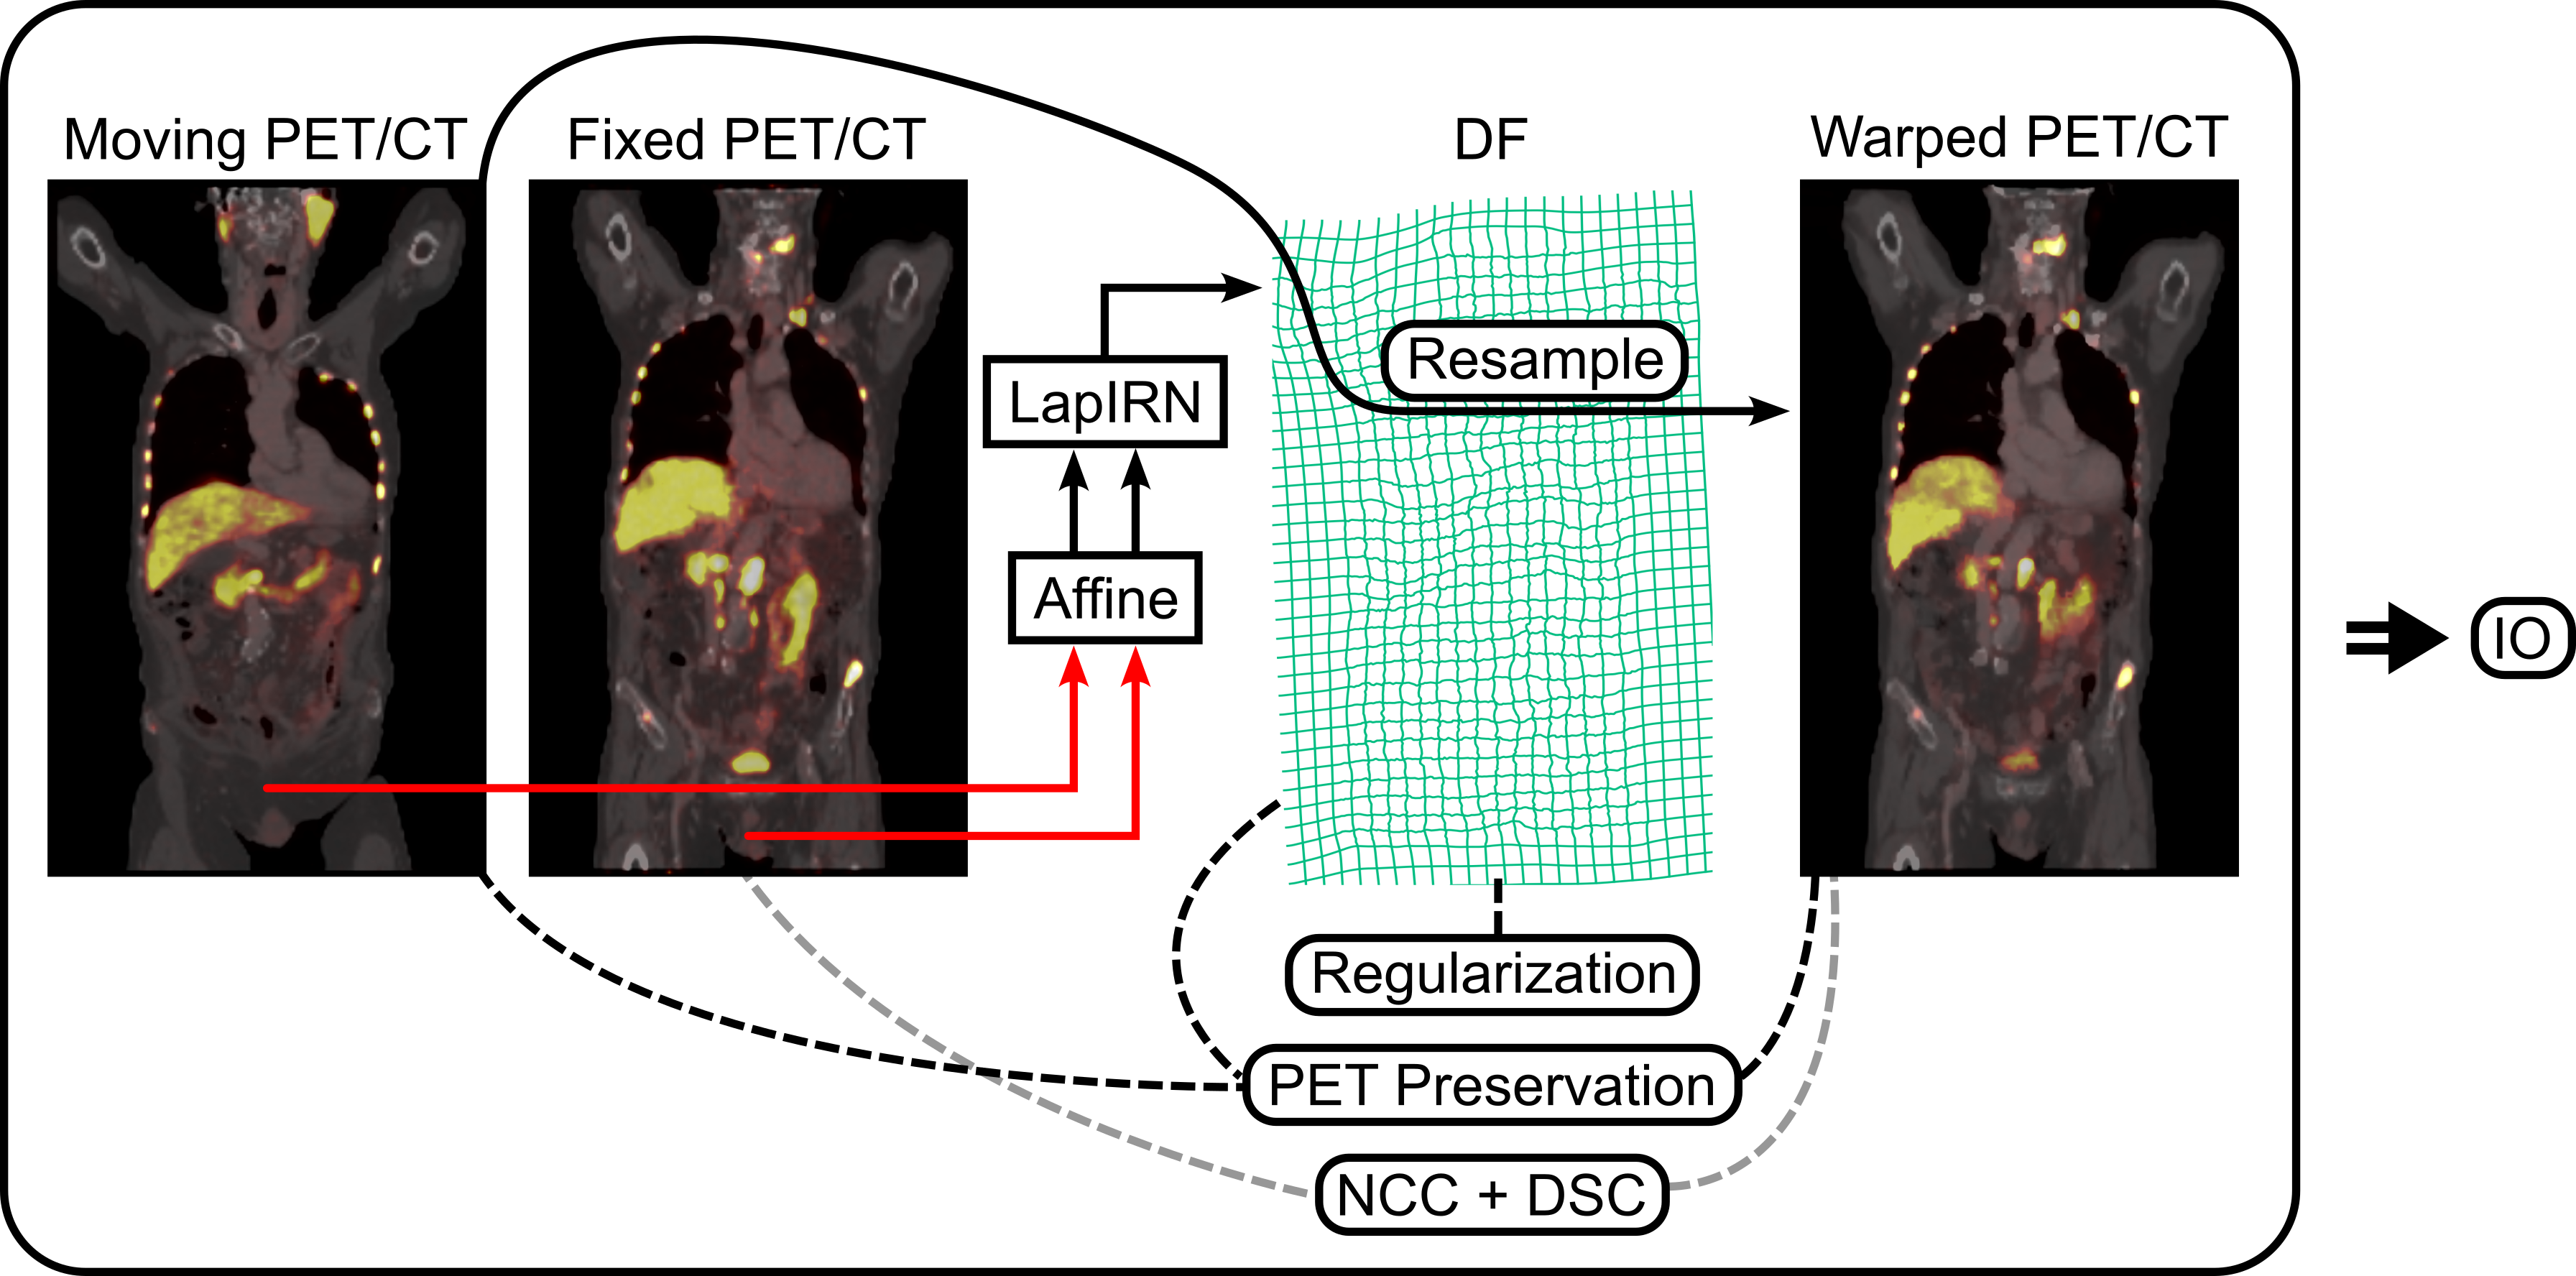
\includegraphics[width=\linewidth]{overview.png}
\caption{Overview of the proposed registration pipeline.
The moving (follow-up) and fixed (baseline) PET/CT scans are first coarsely aligned by an affine pre-registration, and the resulting pair is then passed to the coarse-to-fine LapIRN network, which predicts a dense deformation field (green grid).
Finally, after the LapIRN stage, we refine this field per pair by instance optimization (IO) and resample the moving scan with it into the fixed space (warped PET/CT).
Both stages are driven by the same objective, a weighted sum of three groups of terms: registration accuracy, PET quantification, and deformation regularization (Sec.~\ref{sec:losses}).}
\label{fig:pipeline}
\end{figure}


\section{Methods}

\subsection{Data and Preprocessing}
\label{sec:data_and_preprocessing}

We used the PSMAReg dataset of the Learn2Reg 2026 challenge~\cite{ref_psmareg_challenge}, a longitudinal whole-body PSMA PET/CT cohort in which each subject provides a baseline scan and one or more follow-up scans.
Each scan contains CT and PSMA PET channels; follow-up scans were treated as moving images and baseline scans as fixed images.
The images are provided at $2.7344\times2.7344\times3.27$~mm resolution and cropped to $192\times192\times288$ voxels.
We therefore applied no further geometric preprocessing.
CT was clipped to $[-1000, 1500]$~HU and PET SUV to $[0, 20]$, followed by rescaling to $[0,1]$.

\begin{journaladdition}
We split the 146 labelled challenge training patients with at least two scans into training, validation, and test sets at the patient level, targeting a 70/15/15\% division of registration pairs and balancing the sets for tumour burden and bone versus soft-tissue lesion location.
Training uses all forward pairs of a patient, whereas validation and testing use only follow-up-to-baseline pairs, matching the challenge task.
This yielded 92/26/28 patients and 178/38/38 pairs.
Registration models and the lesion nnU-Net will be trained only on training patients; validation patients will be used for all tuning and model selection.

At test time, TotalSegmentator predictions and predictions from the training-only nnU-Net will supply the labels required by instance optimization (IO).
Provided labels will be reserved for evaluation on test patients and will not enter IO or test-time iterate selection.
\todo{Document the provenance of the provided organ and lesion labels, the segmentation models and their training data, and any dependence between evaluation annotations and predicted labels.}
\end{journaladdition}
Following the ConvexAdam~\cite{ref_convexadam} baseline provided by the challenge organizers, we additionally removed the patient bed and normalized the CT images.




\subsection{Registration Pipeline}
\label{sec:pipeline}
Our pipeline consists of CT-based affine pre-registration, LapIRN-based deformable registration, and optional test-time instance optimization (Fig.~\ref{fig:pipeline}).
Throughout, $I$ denotes the moving PET image, $M$ its lesion mask, $\varphi_{\mathrm{aff}}$ the affine pre-registration, $\varphi_{\theta}$ the network-predicted deformation, and $\varphi$ their composition.
$W$ is the lesion mask warped into the fixed frame.

\subsubsection{Step 1: Affine pre-registration.}
For each pair, ANTs~\cite{ants} estimates an affine transform from the CT images alone, using body masks, CT windowing to $[-1000,1000]$~HU, half-resolution images, and Mattes mutual information.
The transform is converted to a dense displacement field and applied to the moving scan.

\subsubsection{Step 2: Deformable registration.}
The deformable stage uses LapIRN~\cite{ref_lapirn}, with three pyramid levels operating at quarter, half, and full resolution.
Each level predicts a stationary velocity field, adds it to the upsampled velocity from the coarser level, \journal{and exponentiates the result by scaling and squaring to obtain $\varphi_{\theta}$.}
To handle PSMA PET/CT, each sub-network receives four channels: fixed CT and PET, and affinely aligned moving CT and PET.
The similarity loss is computed only on CT, because PET uptake may change after therapy; PET is used as input and in the preservation terms of Sec.~\ref{sec:losses}.
The levels are trained sequentially, with each finer level initialized from the previous one.

\subsubsection{Step 3: Instance optimization.}
At test time, each pair is refined by optimizing a residual stationary velocity field on top of the network prediction.
\begin{journaladdition}
The residual is initialized to zero and exponentiated by scaling and squaring.
The velocity formulation targets diffeomorphic transformations; discrete folding will nevertheless be measured explicitly.
IO will use the objective appropriate to each experimental condition (Sec.~\ref{sec:experiments}).
Its stopping and iterate-selection rule will be chosen on validation patients and frozen before testing; test evaluation labels will not be used to score or select iterates.
\todo{Specify optimized variables, learning rate, iteration budget, and stopping/selection rule, including which predicted-label quantities it may use.}
\end{journaladdition}


\subsection{\journal{Registration Objective}}
\label{sec:losses}
We use a weighted sum of three loss groups, one per evaluation criterion:
\begin{equation}
  \begin{aligned}
    \mathcal{L} = \;
      & \underbrace{\lambda_{\mathrm{NCC}}\,\mathcal{L}_{\mathrm{NCC}}
      + \lambda_{\mathrm{DSC}}\,\mathcal{L}_{\mathrm{DSC}}}_{\text{registration accuracy}} \\
      & + \underbrace{\lambda_{\mathrm{MTV}}\,\mathcal{L}_{\mathrm{MTV}}
      + \lambda_{\mathrm{MTV\text{-}J}}\,\mathcal{L}_{\mathrm{MTV\text{-}J}}
      + \lambda_{\mathrm{jac}}\,\mathcal{L}_{\mathrm{jac}}
      + \lambda_{\mathrm{TLG}}\,\mathcal{L}_{\mathrm{TLG}}}_{\text{PET quantification}} \\
      & + \underbrace{\lambda_{\mathrm{rigid}}\,\mathcal{L}_{\mathrm{rigid}}
      + \lambda_{\mathrm{smooth}}\,\mathcal{L}_{\mathrm{smooth}}
      + \lambda_{\mathrm{NDV}}\,\mathcal{L}_{\mathrm{NDV}}}_{\text{deformation regularization}} .
  \end{aligned}
  \label{eq:total}
\end{equation}
Each group is described below.
All terms are evaluated on the composed transformation $\varphi$.
Only the full-resolution level is trained with the complete objective.
The two coarser levels (quarter and half resolution) use only the similarity, label, and regularization terms; thus $\lambda_{\mathrm{MTV}} = \lambda_{\mathrm{MTV\text{-}J}} = \lambda_{\mathrm{jac}} = \lambda_{\mathrm{TLG}} = \lambda_{\mathrm{rigid}} = 0$.
We omit the PET and bone-specific terms at these resolutions because downsampled lesions and thin ribs span only a few voxels, so volume ratios and per-structure rigid fits mainly reflect interpolation rather than anatomy.

\subsubsection{Registration Accuracy.}
Image similarity is measured using local normalized cross-correlation (NCC), computed as a multi-resolution sum over as many scales as the respective pyramid level has resolutions, i.e.\ one scale at the coarsest and three at the full-resolution level.
NCC is computed on the CT channel only, since PET uptake can change substantially between time points, and a PET similarity term could therefore encourage matching disease-related uptake rather than anatomy.
We additionally use a DSC loss for weak supervision from the CT organ labels.




\subsubsection{Preservation of PET quantification.}

\begin{journaladdition}
PET preservation compares the moving scan before and after transformation, using the same source lesion definition.
For the differentiable training and IO objective, let $\widetilde I=W_{\mathrm{lin}}[I]$ and $\widetilde M=W_{\mathrm{lin}}[M]$ denote the linearly warped PET image and soft lesion mask.
We compute
\begin{equation}
  \mathcal{L}_{\mathrm{MTV}}=
  \left(
  \frac{\left|\sum_x\widetilde M(x)-\sum_xM(x)\right|}{\sum_xM(x)+10^{-5}}
  \right)^2.
  \label{eq:mtv_training_loss}
\end{equation}
\begin{equation}
  \mathcal{L}_{\mathrm{TLG}}=
  \frac{\left|\sum_x\widetilde I(x)\widetilde M(x)-\sum_xI(x)M(x)\right|}
  {\sum_xI(x)M(x)+10^{-5}}.
  \label{eq:tlg_training_loss}
\end{equation}
These losses enter Eq.~\eqref{eq:total} and deliberately differ from the official evaluation metrics of Sec.~\ref{sec:pet_evaluation_metrics}.
Nearest-neighbour mask interpolation is piecewise constant with respect to the displacement and therefore provides no useful gradient for registration; linear interpolation instead supplies a differentiable soft boundary.
The additive denominator stabilizes optimization for empty or very small masks, and squaring the relative MTV error gives a smooth quadratic penalty that emphasizes larger volume errors.
Training uses clipped, normalized PET to keep gradient scales bounded, whereas official TLG evaluation uses PET in SUV units.
\todo{Write the exact equations for the two Jacobian-based PET terms and verify transformation direction, Jacobian convention, reduction, and handling of empty or tiny lesions against the final implementation.}
\end{journaladdition}
All terms are evaluated on the composed transformation $\varphi$ and the original moving lesion mask $M$.

To additionally constrain the deformation within the lesion, we use $\mathcal{L}_{\mathrm{MTV\text{-}J}}$, which penalizes deviations of the mean Jacobian determinant over the warped lesion region $W$ from one.
A third term, $\mathcal{L}_{\mathrm{jac}}$, penalizes per-voxel deviations of the Jacobian determinant from one and therefore discourages local compensating compression and expansion.

\journal{The full-objective condition uses all four PET preservation terms during training and instance optimization; the ablations remove the specified terms.}



\subsubsection{Bone rigidity.}
Many lesions lie within skeletal structures, where rigid motion is physiologically plausible and preserves both volume and intensity ($\det J_{\varphi} = 1$).
\journal{We therefore penalize departures from rigid motion within each skeletal structure.}
For the 61 skeletal TotalSegmentator labels, we fit the displacement of each structure independently with a rigid transformation using closed-form Kabsch alignment~\cite{ref_kabsch,ref_umeyama} and penalize the residual.
This constrains the deformation within each structure while allowing independent motion between structures.


\subsubsection{Deformation regularization.}
We regularize the displacement field using a diffusion term, $\mathcal{L}_{\mathrm{smooth}}$, defined as the mean squared spatial gradient of the displacement, together with a penalty for non-diffeomorphic voxels.
For the latter, we differentiably reproduce the challenge's non-diffeomorphic volume (NDV) metric, which decomposes each voxel into six tetrahedra and accumulates the negative part of their Jacobian determinants over the body mask~\cite{Liu2024}.
The resulting $\mathcal{L}_{\mathrm{NDV}}$ directly corresponds to the scored percentage of non-diffeomorphic volume and provides gradients at the locations where folding occurs.


% Prospective journal protocol; replace planning language after experiments.
\begin{journaladdition}
\subsection{Experimental Design and Model Selection}
\label{sec:experiments}
\label{sec:model_selection}
All experiments below are planned. Settings will be selected on validation patients and frozen before evaluation on test patients.
The split, endpoints, and analysis rules will be fixed before running the core experiments.
\todo{Define the validation selection criterion, sweep ranges, compute budgets, and repeat/seed policy. Do not reuse the previous surrogate-set ranking as journal test evidence.}

\subsubsection{PET and rigidity ablations.}
\begin{itemize}
  \item Train the $2\times2$ conditions: neither PET preservation nor rigidity, PET only, rigidity only, and both. Retain the same registration-accuracy and general regularization terms.
  \item Within the full objective, remove each of $\mathcal{L}_{\mathrm{MTV}}$, $\mathcal{L}_{\mathrm{MTV\text{-}J}}$, $\mathcal{L}_{\mathrm{jac}}$, and $\mathcal{L}_{\mathrm{TLG}}$ individually.
  \item Prioritize matched training for the central claims. Specify each condition's training and IO objective separately; identify any IO-only ablation as such.
  \item Report paired effects of PET, rigidity, and their combination on alignment, lesion preservation, and deformation quality; include the PET--rigidity interaction if estimable under the chosen analysis.
\end{itemize}

\subsubsection{Comparison of rigidity penalties.}
Compare no rigidity, Staring with all three components~\cite{ref_rigidity_3_staring}, Staring with mask erosion, and the existing Kabsch rigid-fit penalty~\cite{ref_kabsch}.
Tune or sweep each method's weight separately; equal numerical weights need not imply comparable constraint strength.
\begin{itemize}
  \item Document the three Staring components, their scaling, derivative stencils, boundary handling, and coordinate units. Specify the erosion rule and report bones/voxels retained.
  \item Use alignment versus physical within-bone distance distortion as the main comparison, with folding alongside. Report bone rigidity error (BRE) only as a secondary endpoint because it closely matches the Kabsch objective.
  \item Measure direct stencil leakage separately from the effect on surrounding tissue. Kabsch avoids direct stencil leakage, but shared deformation parameters and regularization can still influence soft tissue.
  \item Scope conclusions to the tested resolutions, implementations, and weight ranges.
\end{itemize}

\subsubsection{Accuracy--preservation trade-off.}
Run a small PET-weight sweep including zero and the current setting.
\todo{Specify whether one multiplier scales the whole PET group, which relative term weights remain fixed, and whether each setting is retrained or changes IO only.}
Plot alignment against lesion preservation and report deformation quality for every setting.
Select operating points on validation patients and evaluate frozen settings on the test partition, without choosing a preferred setting from test results.

\subsubsection{Baselines.}
\label{sec:baselines}
Re-evaluate the initial alignment, affine registration, NiftyReg~\cite{MODAT2010,modat2014}, and ConvexAdam~\cite{ref_convexadam} on the new test partition under the same evaluation definitions.
Report the full method with and without IO.
\todo{Freeze baseline configurations, validation tuning allowances, and runtime measurement. The previous container and surrogate-validation configurations are not journal comparison groups.}

\subsection{Evaluation Endpoints and Statistical Analysis}
\label{sec:evaluation}
\begin{itemize}
  \item \textbf{Alignment:} per-bone and soft-tissue organ Dice and surface distance; near-bone landmarks only if independently available. Define aggregation over structures and handling of absent or truncated anatomy.
  \item \textbf{PET preservation:} aggregate and per-lesion MTV/TLG change from the original moving scan to that same scan after warping. Report signed, absolute, and upper-tail errors, stratified by bone association and lesion size.
  \item \textbf{Lesion measurement:} define lesions on the source scan and track them through the transformation. Predefine size bins, bone-association rules, minimum denominators, empty-mask handling, field-of-view exclusions, SUV units, and interpolation. Distinguish resampling effects from deformation effects using a specified control.
  \item \textbf{Bone shape:} measure distortion of sampled within-bone point-pair distances in physical coordinates, covering short and long distances. Predefine sampling, distance bins, and normalization; report BRE secondarily.
  \item \textbf{Deformation quality:} report NDV/folding inside bones, in an outside boundary band, and across the body. Specify masks, band width in physical units, denominators, and consistent units.
  \item \textbf{Boundary mechanism:} quantify the fraction of stencil samples outside bone and the fraction of bones/voxels retained after erosion. State how bones that disappear after erosion are handled.
  \item \textbf{Uncertainty:} report paired method effects with patient-level confidence intervals, accounting for multiple pairs and lesions per patient. A candidate is patient-cluster bootstrap resampling that retains all within-patient observations and method pairing.
\end{itemize}
\todo{Freeze primary endpoints and contrasts, the upper-tail statistic, patient weighting, uncertainty procedure, and multiplicity handling before test evaluation. Report evaluable patient/pair/lesion counts and exclusions.}

\subsection{Optional Supporting Analyses}
\label{sec:optional}
\begin{itemize}
  \item \textbf{Gradient analysis:} one loss-pair cosine matrix, selected IO trajectories, and representative maps. Distinguish displacement-space maps from gradients in optimized velocity coordinates; mask near-zero gradients and report weighted magnitudes. Local cosine similarity is not evidence of a final performance trade-off.
  \item \textbf{External cohort:} include only if feasible. Combine automatic measurements with blinded, randomized clinician review; add sparse landmarks if available. Separate IO labels from independent evaluation. Distinguish resampling from deformation effects.
\end{itemize}
These analyses are optional; independent evaluation and the core experiments take priority.
\end{journaladdition}


\subsection{Implementation Details}
\label{sec:infrastructure}
Augmentations were chosen to mimic longitudinal variability: left--right flipping ($p=0.5$), CT intensity shifting by $\pm0.02$ in the normalized window (about $\pm50$~HU), CT scaling from $0.9$ to $1.1$, and PET scaling from $0.85$ to $1.15$ without additive shifts.
To simulate a field-of-view mismatch, we crop up to 40 axial slices from either end of both scans, followed by independent moving and fixed crops of up to 10 additional slices.

\begin{journaladdition}
\paragraph{Training configuration to confirm.}
The previous pipeline used sequential Adam training for $60$k, $60$k, and $120$k steps, learning rates of $3\cdot10^{-4}$, $2\cdot10^{-4}$, and $2.5\cdot10^{-4}$, batch size one, and gradient accumulation over four steps.
These are starting settings for retraining, not completed experiments.
\begin{itemize}
  \item Confirm the warmup and coarse-level freezing schedule, augmentations, loss weights, and random seeds. Keep the training budget and shared settings matched across central ablations.
  \item Record mixed precision, transformation precision, final software versions, hardware, training time, and per-pair inference/IO time for the new runs.
  \item Confirm which pyramid levels use PET and rigidity terms in each condition.
\end{itemize}
\end{journaladdition}

\section{\journal{Results}}
\begin{journaladdition}
\noindent\textit{Journal draft: experiments are pending. All tables and figures below are planned outputs, not findings. The previous evaluation and leaderboard results have been removed because they used a different protocol.}

\subsection{Independent-Test Comparison}
\begin{itemize}
  \item Report the final cohort, exclusions, and evaluable structures/lesions.
  \item Compare baselines and the full model with and without IO on the frozen test partition (Table~\ref{tab:journal_baselines}).
  \item Add paired patient-level effects and uncertainty; describe alignment, preservation, folding, and runtime without selecting a winner from test results.
\end{itemize}
\end{journaladdition}
\begin{table}[htbp]
\journalcolor
\centering
\caption{\journal{Planned independent-test comparison. All entries are pending; ``pending'' is not a numerical result. Report patient-level uncertainty and paired effects in the final table/text. Per-lesion and regional endpoints are detailed separately.}}
\label{tab:journal_baselines}
\scriptsize
\setlength{\tabcolsep}{3pt}
\begin{tabular}{lccccc}
\toprule
Method & Dice & HD95 & MTV/TLG & NDV & Runtime \\
\midrule
Initial & pending & pending & pending & pending & pending \\
Affine & pending & pending & pending & pending & pending \\
NiftyReg & pending & pending & pending & pending & pending \\
ConvexAdam & pending & pending & pending & pending & pending \\
Full model, no IO & pending & pending & pending & pending & pending \\
Full model + IO & pending & pending & pending & pending & pending \\
\bottomrule
\end{tabular}
\end{table}


\begin{journaladdition}
\subsection{Separate and Combined Effects of PET Preservation and Rigidity}
\label{sec:ablation}
\begin{itemize}
  \item Fill the matched-training $2\times2$ comparison and the four PET-term removal conditions (Table~\ref{tab:journal_ablations}).
  \item Report aggregate versus per-lesion changes; check whether aggregate cancellation hides large individual errors.
  \item Show signed, absolute, and upper-tail errors by lesion size and bone association (Fig.~\ref{fig:journal_lesions}).
\end{itemize}
\end{journaladdition}
\begin{table}[htbp]
\journalcolor
\centering
\caption{\journal{Planned matched-training ablations. Accuracy and general regularization terms are retained. The endpoint groups are alignment, aggregate/per-lesion PET preservation, and deformation quality. Results and patient-level paired effects are pending; any additional IO-only ablations must be reported separately.}}
\label{tab:journal_ablations}
\small
\setlength{\tabcolsep}{4pt}
\begin{tabular}{lccc}
\toprule
Condition & PET terms & Rigidity & Results \\
\midrule
Neither & None & Off & Pending \\
PET only & All four & Off & Pending \\
Rigidity only & None & On & Pending \\
Both (full) & All four & On & Pending \\
\midrule
Full minus $\mathcal{L}_{\mathrm{MTV}}$ & Other three & On & Pending \\
Full minus $\mathcal{L}_{\mathrm{MTV\text{-}J}}$ & Other three & On & Pending \\
Full minus $\mathcal{L}_{\mathrm{jac}}$ & Other three & On & Pending \\
Full minus $\mathcal{L}_{\mathrm{TLG}}$ & Other three & On & Pending \\
\bottomrule
\end{tabular}
\end{table}

\begin{figure}[htbp]
\journalcolor
\centering
\figplaceholder{0.18}{Planned panels: aggregate versus per-lesion MTV/TLG error; signed and absolute error distributions; upper-tail summaries by lesion size and bone association.}
\caption{\journal{Planned lesion-preservation analysis for the matched PET and rigidity ablations. Compare each moving scan before and after warping, with patient-level uncertainty. State subgroup counts and the predeclared upper-tail statistic. No experimental data are shown.}}
\label{fig:journal_lesions}
\end{figure}


\begin{journaladdition}
\subsection{Rigidity Comparison and Boundary Effects}
\begin{itemize}
  \item Compare each rigidity method over its own weight range: bone/organ alignment, distance distortion, regional folding, and secondary BRE.
  \item Relate stencil leakage and erosion retention to the observed outcomes without assuming a mechanism in advance (Fig.~\ref{fig:journal_rigidity}).
  \item Include representative bone-boundary examples under a documented case-selection rule.
\end{itemize}
\end{journaladdition}
\begin{figure}[htbp]
\journalcolor
\centering
\figplaceholder{0.18}{Planned panels: bone/organ alignment versus physical distance distortion over method-specific weights; folding inside bone and in the outer band; stencil leakage and erosion retention; representative boundary maps.}
\caption{\journal{Planned comparison of no rigidity, Staring, Staring with erosion, and Kabsch. Report regional folding alongside alignment and distance distortion, and show boundary-mechanism measurements separately. BRE is secondary. No experimental data are shown.}}
\label{fig:journal_rigidity}
\end{figure}


\begin{journaladdition}
\subsection{Accuracy--Preservation Trade-off}
\begin{itemize}
  \item Show the predeclared PET-weight settings and their patient-level uncertainty (Fig.~\ref{fig:journal_tradeoff}).
  \item Identify the validation-selected operating point and report its frozen test performance.
  \item Discuss whether preservation changes alignment or folding, including heterogeneous lesion responses.
\end{itemize}
\end{journaladdition}
\begin{figure}[htbp]
\journalcolor
\centering
\figplaceholder{0.18}{Planned panels: alignment versus per-lesion MTV and TLG preservation across a small PET-weight sweep, including zero and the current setting; corresponding deformation quality.}
\caption{\journal{Planned accuracy--preservation trade-off. Mark the operating point selected on validation patients and distinguish validation curves from frozen-setting test results. Include patient-level uncertainty and identify whether settings change matched training or IO only. No experimental data are shown.}}
\label{fig:journal_tradeoff}
\end{figure}


\begin{journaladdition}
\subsection{Optional Supporting Results}
\todo{Include gradient analysis and/or external-cohort results only if completed; otherwise remove this subsection. Do not imply external validation from surrogate measurements alone.}
\end{journaladdition}

\section{\journal{Discussion}}
\begin{journaladdition}
\noindent\textit{Discussion outline; replace with evidence-based interpretation after the core experiments.}
\begin{itemize}
  \item \textbf{Main answer:} summarize the separate and combined effects of PET preservation and bone rigidity, with the principal effect sizes and uncertainty.
  \item \textbf{Lesion quantification:} explain whether aggregate preservation conceals per-lesion errors, which lesion groups benefit, and whether any groups show worse upper-tail errors. Preserving a warped scan's quantification does not establish clinical response accuracy or imply unchanged disease across time.
  \item \textbf{Rigidity:} interpret alignment versus distance distortion alongside folding and soft-tissue effects. Discuss stencil leakage and erosion retention only to the extent supported by the measurements. Avoid claiming a new rigidity method or general superiority beyond the tested setting.
  \item \textbf{Trade-off:} explain the practical consequences of the PET-weight sweep and how validation-only selection determines the reported operating point.
  \item \textbf{Evaluation validity:} discuss prior patient exposure, label provenance, possible dependence between predicted and evaluation labels, and uncertainty with repeated pairs/lesions. State any limitations of the independent test partition that remain after retraining.
  \item \textbf{Practical limitations:} low resolution, small lesions and thin bones, interpolation and field-of-view effects, segmentation dependence, and compute/runtime. Separately interpolating PET and a nearest-neighbour lesion mask introduces a non-zero, subvoxel-phase-dependent TLG error even for rigid translations. Because the same estimator enters the optimization objective, the model can reduce the measured interpolation error through its deformation; such a reduction must not automatically be interpreted as improved physical biomarker preservation. Interpret effects relative to the resampling control, and do not assume theoretical diffeomorphism eliminates discrete folding.
  \item \textbf{Scope and generalization:} distinguish the core labelled-cohort evidence from optional gradient analyses and external-cohort evidence, if available.
\end{itemize}
\paragraph{Conclusion to write after evaluation.}
\todo{State what the independent evaluation supports about alignment, lesion preservation, and bone rigidity, including the main trade-off and remaining limitation.}
\end{journaladdition}


\begin{credits}
\subsubsection{\ackname}

\subsubsection{\discintname}
The authors have no competing interests to declare that are relevant to the content of this article.

\end{credits}
%
% ---- Bibliography ----
%
% BibTeX users should specify bibliography style 'splncs04'.
% References will then be sorted and formatted in the correct style.
%
% \bibliographystyle{splncs04}
% \bibliography{mybibliography}
%
\bibliographystyle{splncs04-etal}
\bibliography{references}


\end{document}
